\section{4+1 view architecture} \label{title:viewArc}
Denne model beskriver arkitekturen af software baserede systemer. For at skabe en fyldestgørende gennemgang af systemet gøres brug af fire forskellige synsvinkler. Disse synsvinkler har til formål at  tilfredsstille alle interessenter og sørge for at alle parter forstår systemet. Eksempler på parter kunne være kunden, projektleder eller udviklere. Med udgangspunkt i use cases består modellen af følgende punkter: 

\begin{figure}[H]
	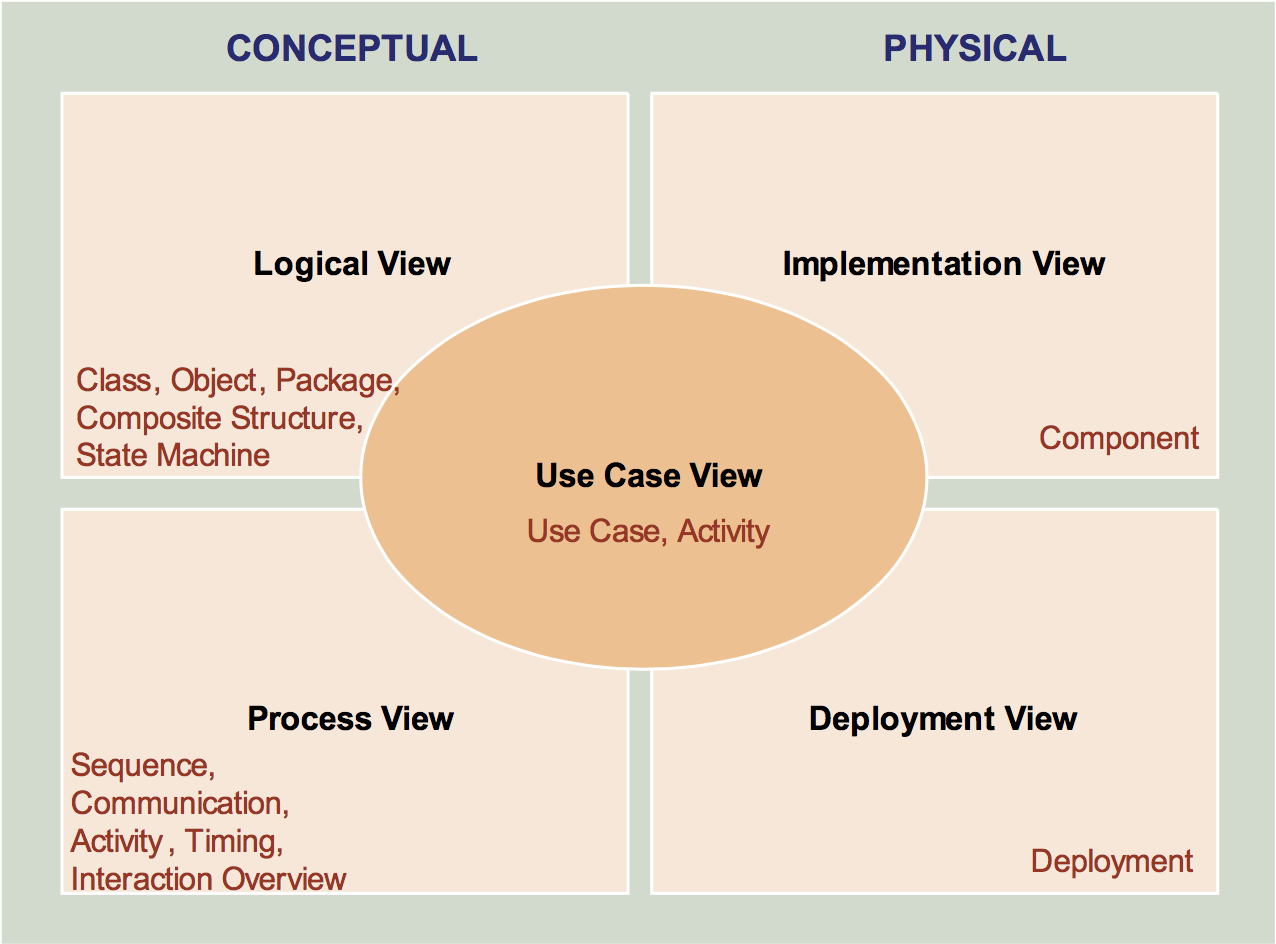
\includegraphics[width=\textwidth]{SystemArkitektur/filer/4plus1model.png}
	\caption{4+1 view architecture model}\label{fig:4plus1model}
\end{figure}

\textit{Logical view:} Denne synsvinkel beskriver systemets funktionalitet via centrale elementer, mekanismer og stadier.

\textit{Process view:} Beskæftiger sig med de dynamiske aspekter af systemet, forklarer system processer, hvordan de kommunikerer, og fokuserer på systemets opførsel i drift.

\textit{Implementation view:} Denne vinkel involverer udviklerens perspektiv og beskæftiger sig med hvordan software implementeres.

\textit{Deployment view:} Beskriver systemet fra en fysisk synsvinkel, blandt andet hvordan eksekveringen af softwares skal foregå på apparatet og hvordan systemets fysisk setup skal ser ud. 

Modellen “\textit{4+1 view architecture}” er beregnet primært til software baserede udviklingsprojekter og derfor bruges den som en retningslinje og inspiration til systemet arkitekturen. Da Konditioneringsapparatet er en prototype som involvere både hardware og software er modellen blevet tilpasset dertil. Endvidere vil systemet blive præsenteret og gennemgået ved hjælp af SysML standarden, selvom modellen er lavet til UML.

